Viele Jahre wissenschaftlicher und technologischer Fortschritt haben zur Entwicklung des Quantenbits, kurz \textit{Qubit} beigetragen. Genau wie das klassische Bit, die kleinste Ma\ss einheit zur Darstellung von Informationsgehalt, kann auch das Quantenbit die Zust\"ande 1 und 0 annehmen. Wesentlicher Unterschied zu einem klassischen Bit ist, dass es sich bei einem Qubit um ein Zweizustandssystem handelt, d.h. es kann sich zu einer gewissen Wahrscheinlichkeit in einem dieser beiden Zust\"ande 1 oder 0 befinden. Hierbei ist wichtig, dass der Zustand dieses Quantenbits nur dann in Erfahren gebracht werden kann, indem es gemessen wird.\\
Um den Zustand eines Qubits darzustellen, werden Zustandsvektoren genutzt. Um diese Zust\"ande mathematisch zu veranschaulichen wird die sogenannte Dirac Noation $|\rangle$ genutzt, diese ist die standard Notation, um in der Quantenmechanik Zust\"ande darzustellen.
\begin{equation} \label{eqn:first}
        |0\rangle = \begin{bmatrix}
        1 \\
        0 \\
        \end{bmatrix}
        \,\,\, \,\,\,
        |1\rangle = \begin{bmatrix}
        0 \\
        1 \\
        \end{bmatrix}
\end{equation}
Somit zeigt \ref{eqn:first} die Basiszust\"ande \textit{(Computational basis state)} $|0\rangle$ und $|1\rangle$, welche eine orthogonale Basis bilden \cite{nielsen_chuang_2010}. Es ist jedoch auch m\"oglich, dass sich ein Quantenbit in einem Zustand befindet, der sich von diesen beiden unterscheidet.
\begin{equation}\label{eqn:superposition}
\begin{gathered}
        |\psi\rangle = \alpha |0\rangle+\beta |1\rangle = \begin{bmatrix}
        \alpha \\
        \beta \\
        \end{bmatrix} \qquad \alpha, \beta \in \mathbf{C}
        \end{gathered}
\end{equation}
Das hei\ss t auch Linearkombinationen k\"onnen aus diesen Zust\"anden gebildet werden \ref{eqn:superposition}. Dies wird als Superpostion oder auch \"Uberlagerung bezeichnet, wobei $\alpha$ und $\beta$ die Amplituden des Zustands $|\psi\rangle$ darstellen \cite{nielsen_chuang_2010}. \\
Um zu erfahren, zu welcher Wahrscheinlichkeit sich ein Quantenbit in einem bestimmten Zustand befindet, muss das Qubit gemessen werden. F\"ur den Zustandsvektor $|\psi\rangle$ erh\"alt man somit nach der Messung, mit der Wahrscheinlichkeit $|\alpha|^2$ das Ergebnis 0, und mit der Wahrscheinlichkeit $|\beta|^2$ das Ergebnis 1 \cite{nielsen_chuang_2010}.
\begin{equation}\label{eqn:messung}
        \begin{gathered}
                p(|0\rangle) = |\langle 0|\psi \rangle|^2 \\
                \Rightarrow | \alpha \langle 0|0 \rangle|^2 + |\beta \langle 0|1 \rangle |^2 \\
                = | \alpha |^2
        \end{gathered}       
\end{equation}
Die Messung wird durchgef\"uhrt, indem das innere Produkt \"uber den Zustandsvektor und den zugeh\"origen Basiszustand gebildet und quadriert wird \ref{eqn:messung}. Um eine Wahrscheinlichkeit von 1 zu gew\"ahrleisten, muss der Zustandsvektor normalisiert sein. Somit muss \ref{eqn:normalisierung} f\"ur den Zustandsvektor gelten.
\begin{equation}\label{eqn:normalisierung}
\begin{gathered}
         \langle \psi | \psi \rangle = 1 \\
         \Rightarrow |\alpha|^2 +|\beta|^2 = 1
\end{gathered}
\end{equation}
Vor der Messung eines Qubits kann es sich in einem Kontinuum an Zust\"anden zwischen $|0\rangle$ und $|1\rangle$ befinden \cite{nielsen_chuang_2010}. Das erm\"oglicht einem Quantenbit, sich in den Zust\"anden $|0\rangle$ und $|1\rangle$ gleichzeitig zu befinden. Auf diesen Zustandsvektor wird oft zur\"uckgegriffen, \ref{eqn:+state} soll diesen verdeutlichen.
\begin{equation}\label{eqn:+state}
|+\rangle = \frac{1}{\sqrt{2}}|0\rangle+\frac{1}{\sqrt{2}}|1\rangle
\end{equation}
Da der Zustandsvektor normalisiert sein muss \ref{eqn:normalisierung}, ist es m\"oglich die allgemeine Darstellung eines Quantenbits \ref{eqn:superposition} mit Hilfe des Additionstheorems $\sqrt{\sin(x)^2+\cos(x)^2} = 1$ zu vereinfachen.
\begin{equation}\label{eqn:bloch-kugel}
\begin{gathered}
|\psi\rangle = \cos\left(\frac{\theta}{2}\right)|0\rangle+e^{i\phi}\sin\left(\frac{\theta}{2}\right)|1\rangle \qquad \theta, \phi \in \mathbf{R}
\end{gathered}
\end{equation}
Zustandsvektor $|+\rangle$ l\"asst sich somit durch $\phi= 0$ und $\theta = \frac{\pi}{2}$ darstellen. \ref{eqn:bloch-kugel} wird als Blochvektor bezeichnet, jeder Blochvektor l\"asst sich als Punkt auf einer dreidimensionalen Kugel (Bloch-Kugel) durch die Kugelkoordinaten $\phi$ und $\theta$ mit einem Radius von $r = 1$ darstellen.
\begin{figure}[h]
\centering
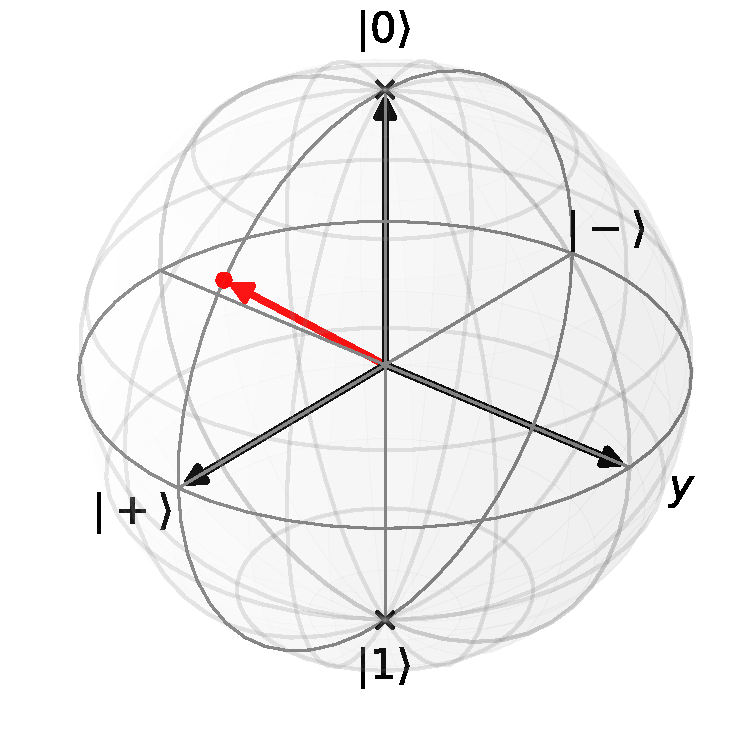
\includegraphics[width=0.7\textwidth]{figures/blochsphere.pdf}
\caption{Darstellung von Quantenbits innerhalb der Bloch-Kugel}
\label{fig:Bloch-Kugel}
\end{figure}
Die Bloch-Kugel ist ein Unterraum des Hilbertraums. Jede Linearkombination zul\"assiger Vektoren innerhalb dieses Unterraums bilden wieder einen zul\"assigen Vektor, daher gibt es unendlich viele Punkte auf der Bloch-Kugel.
